\chapter{Structural Specification}
\label{ch:Appendix C}
The structural specification is a format and application independent data model
specification of the formal specification of IMF. The structural specification aims to faithfully represent the
intentions of the formal specification while also including the specification of how, e.g., objects metadata and
attributes and attribute values are represented, which the formal specification does not contain. The purpose of the
structural specification is to be a common language and format for developing concrete serialization formats for IMF
and serve as documentation for application developers.

\begin{figure}[htb]
  \centering
  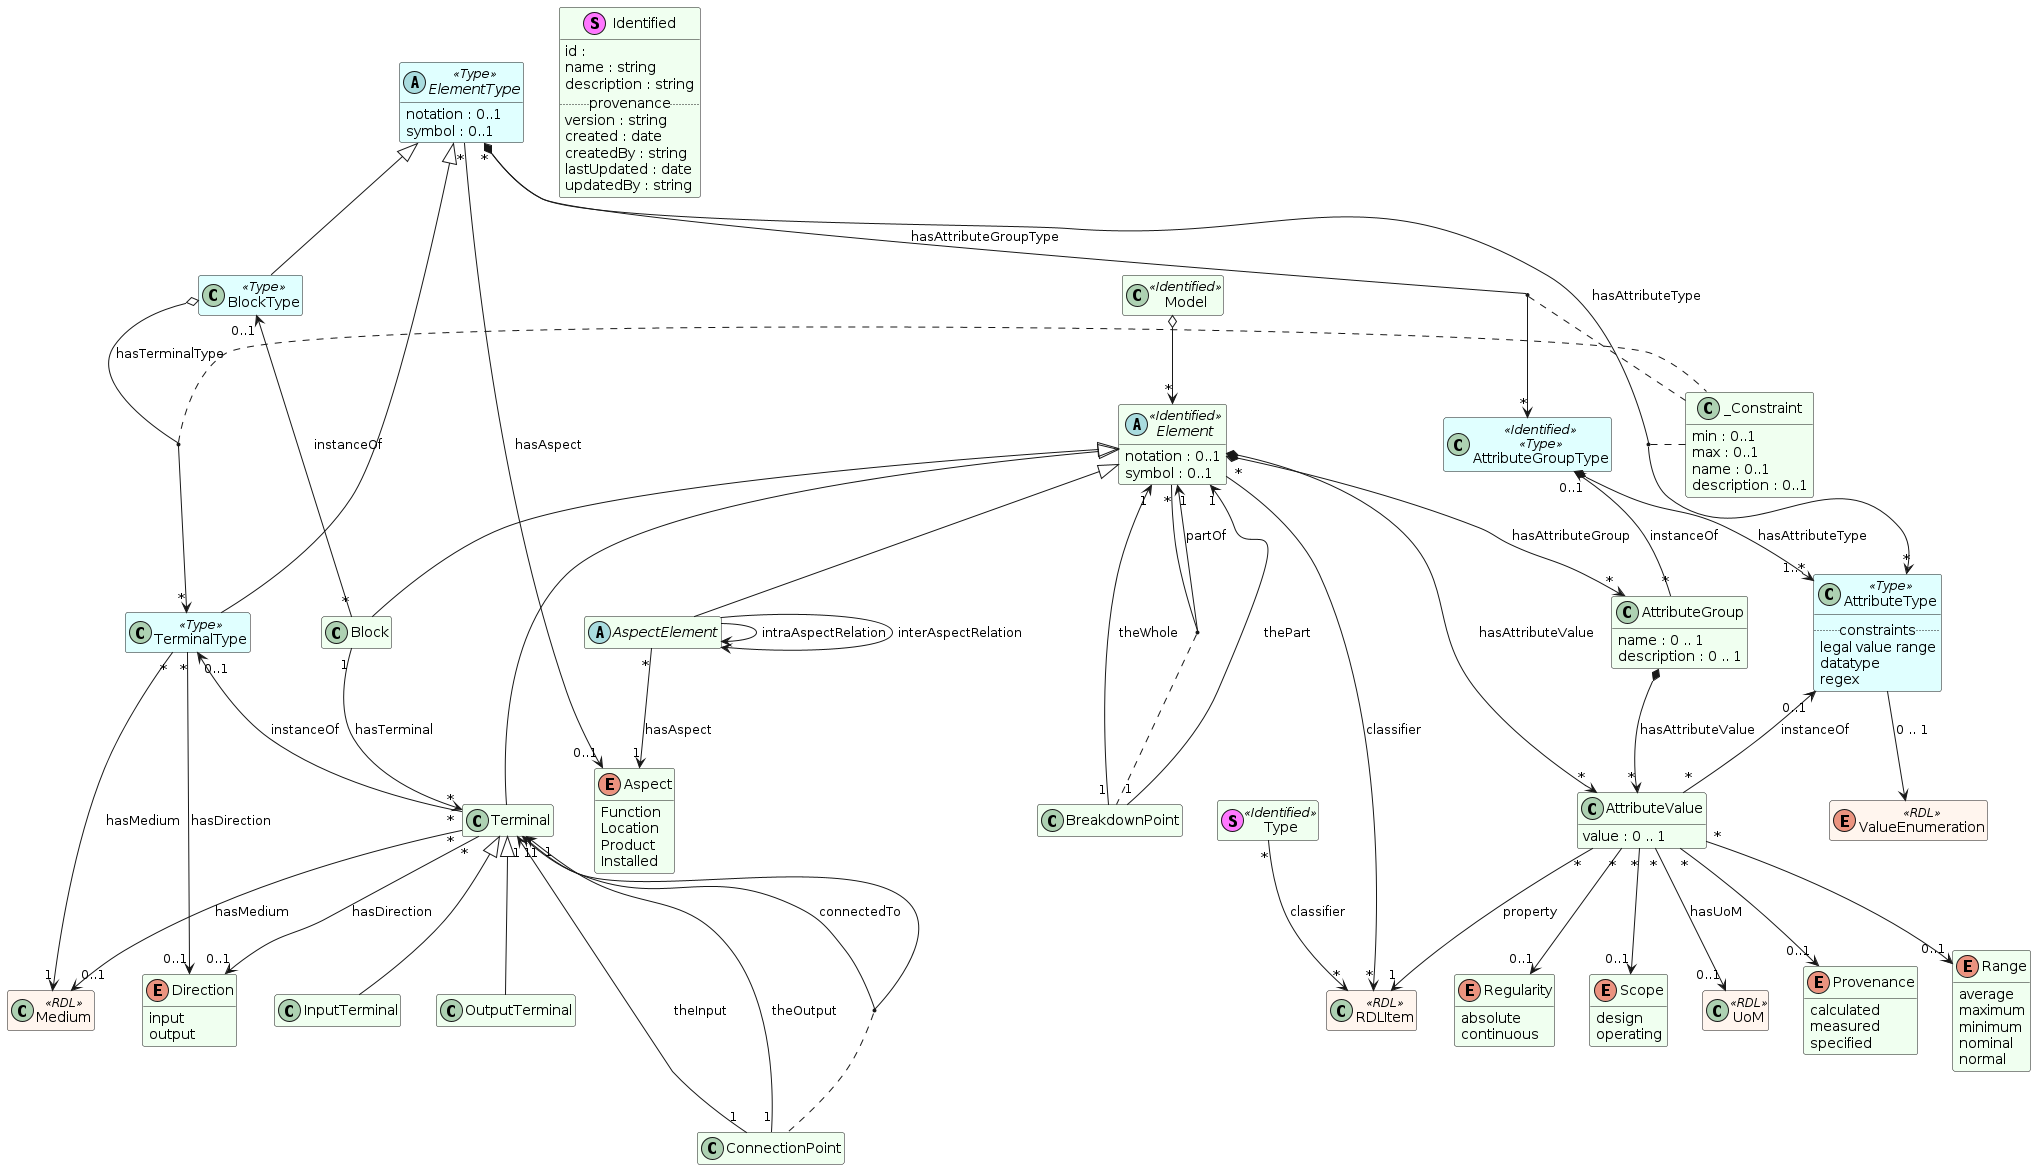
\includegraphics[width=1\textwidth]{img/IMFmanual-img073.png}
  \caption{The complete structural specification.}
  \label{fig:Figure 55}
\end{figure}